\section{Experiments}
\label{sec:expts}
About 10 experiments have been performed using SBHS locally while about 5 of them through remote access.  The open loop experiments are not affected much with a moderate amount of network traffic.  However, key learning is while implementing the control algorithms and observing the effect of network delay.  The results of a few experiments are presented next.

\subsection{Identification using step response data}
As reported in \cite{ia010}, the step test experiment has been conducted by giving 2 step changes of 5 PWM units each and allowing the temperature profile to stabilize each time.  The process model is then identified using this step response data
\cite{karl95,seborg04}. Notably, the remotely performed experiments reported in this paper are done on the same unit reported in \cite{ia010}.  

For the given two step changes, we got the following models \cite{ia010}:
\begin{align*}
G_1 &= \frac{0.62}{44s + 1}e^{-10s}, \ 
G_2 = \frac{0.65}{50s + 1}e^{-10s}
\end{align*}


\subsection{PID control}
The efficacy of the PID controller, in discrete form, is explored next.
\begin{align}
u(t) = K\left[e(t) + \frac{1}{\tau_i} \int_0^t e(t)\,dt + \tau_d
  \frac{de(t)}{dt}\right] 
\end{align}

With the data acquired after every $T_s$ seconds, the integral and derivative terms can be approximated as,
\begin{align}
\int_0^t e(t)\,dt & \approx T_s \sum_{i=0}^{t} e(i) \\ 
\frac{de(t)}{dt} & \approx \frac{e(t) - e(t-1)}{T_s} 
 \end{align}

Using the reaction curve method for the models of the two step response experiments stated earlier,  we arrive at the following values: 

\begin{align*}
L_1 = 10, \tau_1 &= 90, K_1 = 0.62 \\
L_2 = 10, \tau_2 &= 105,K_2 = 0.65
\end{align*}


\subsubsection{Local implementation}
This experiment implements the PID controller locally i.e. the user has a unit connected to his/her computer.

Using the first set and the relations $K_p=0.9/RL$,
$\tau_i=3L$, we arrive at:
\begin{align*}
u & = \text{ubias} + K_p\left[\text{et} +
  \frac{\text{eti*Ts}}{\tau_i}\right] \\ 
K_p & = 13.06, \tau_i = 30 \\
\text{et} & = \text{setpoint - temp, eti = eti + et}
\end{align*}
 
where eti is the accumulated error.  The response for this controller
is depicted in Fig. \ref{fig:pid-2}.  This has been described in greater detail in \cite{ia010}.

\begin{figure}
\hspace{-0.2in}
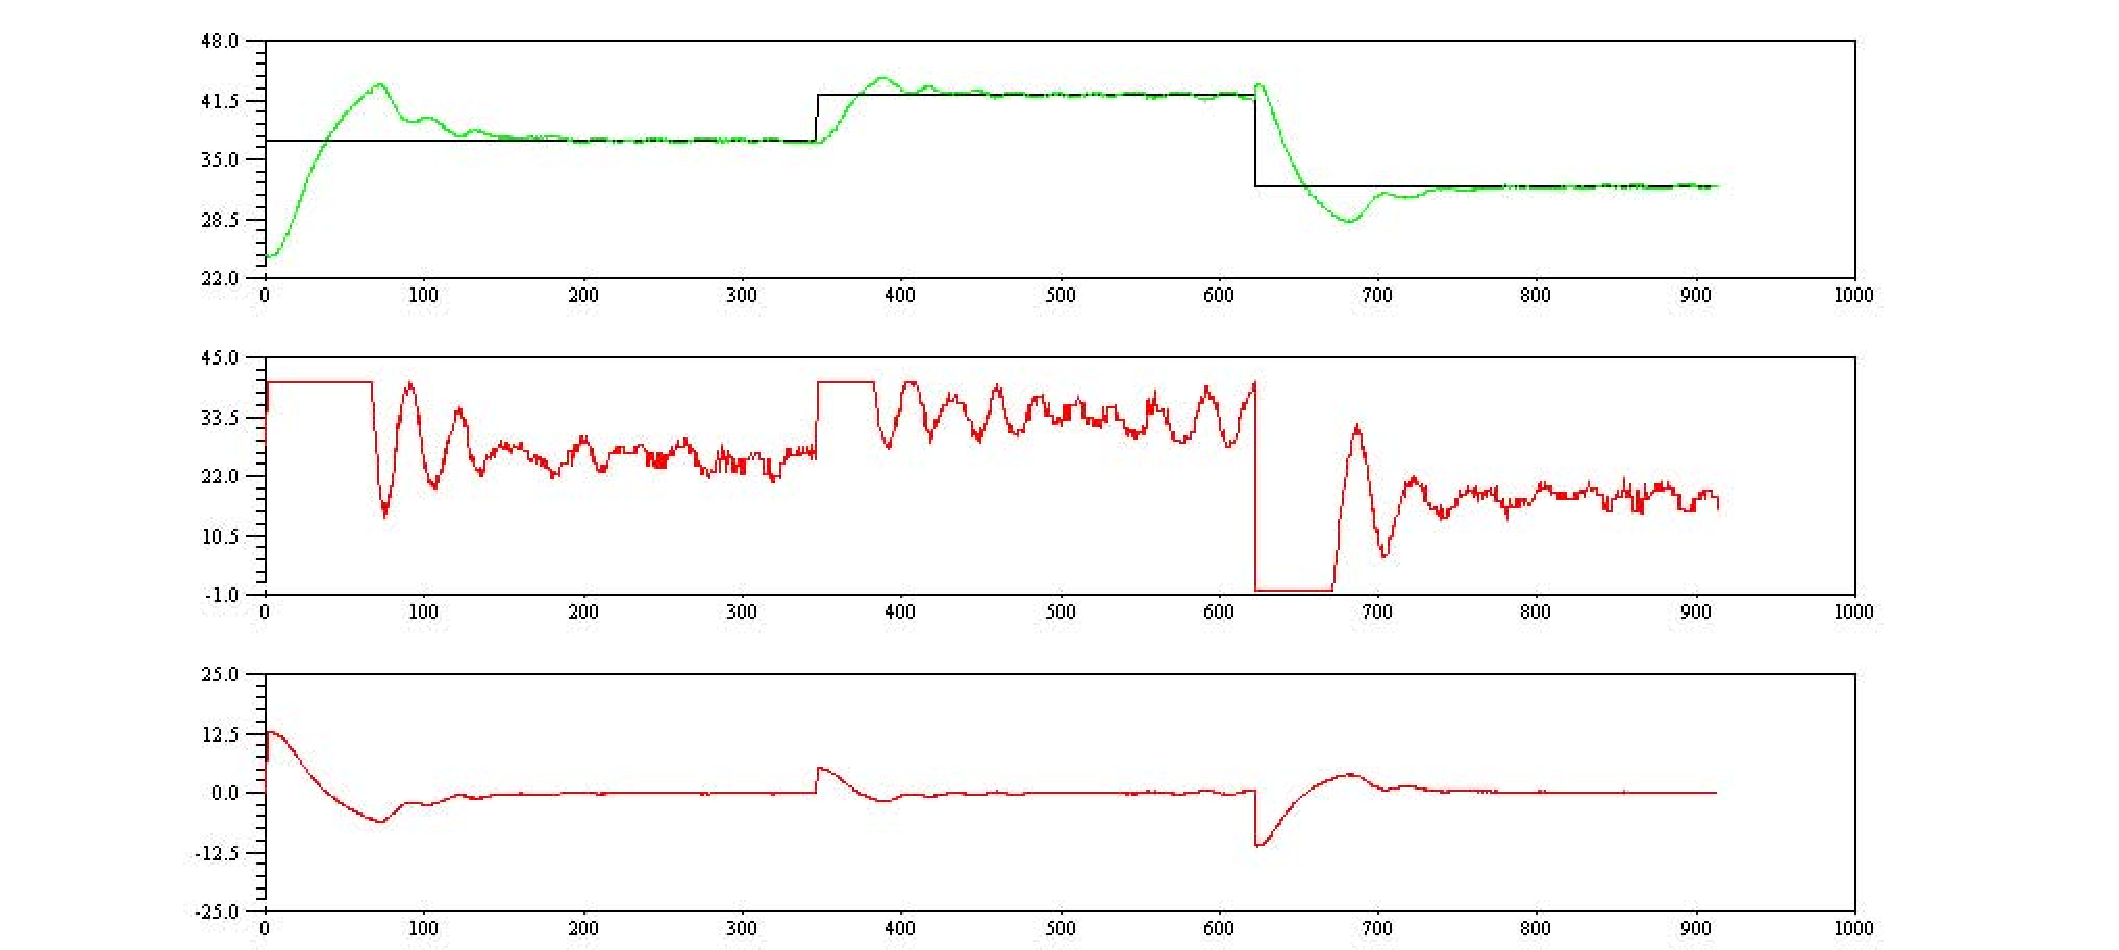
\includegraphics[width=1.2\linewidth]{figures/pi-1}
\caption{Local PI controller implementation: temperature, heater duty,
  error} 
\label{fig:pid-2}
\end{figure}


\subsubsection{Over intranetwork}
The control effort for the same implementation but over network is found to be oscillatory.  The experimental result is depicted in figure \ref{fig:pidosc}.  Next, we re-tune the controller to get better results.

\begin{figure}
\hspace{-0.2in}
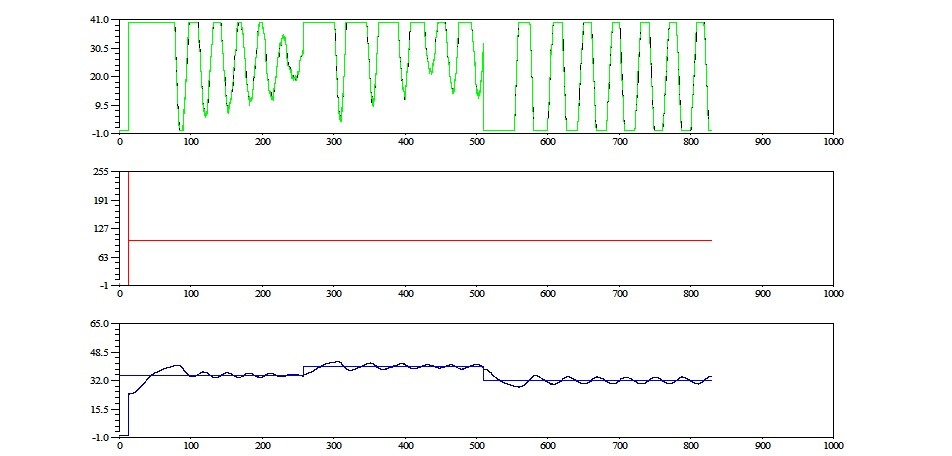
\includegraphics[width=1.2\linewidth]{figures/pidc_intra_osc}
\caption{PID control with local PID tuning parameters and remote
  implementation: heater duty, fan speed, temperature}
\label{fig:pidosc}
\end{figure}

%Tightly tuned real time PID control
In order to implement an acceptable control algorithm, we either need to compensate for time delay or tightly tune the controller.  The source of time delay is network traffic.  With multiple applications running on the same machine and the sampling done every 0.4 s, a small amount of time is also spent in reading from and writing to a file at both the ends.

We implemented the controller with the tuning parameters, $K_p = 2$, and $\tau_i = 50$.  The real implementation results are shown in figure \ref{fig:pidctun}.  The tracking is found to be satisfactory.

\begin{figure}
\hspace{-0.2in}
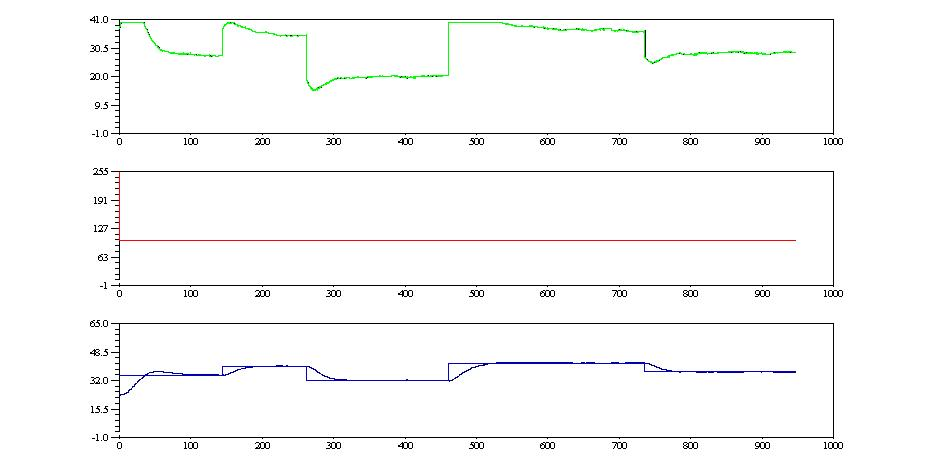
\includegraphics[width=1.2\linewidth]{figures/pidc_intra}
\caption{Tuned PID controller and remote implementation: heater duty,
  fan speed, temperature}
\label{fig:pidctun}
\end{figure}

The possibility of real-time control using a disturbance observer
\cite{kempf96,jones07} is being explored. 
